% GNUPLOT: LaTeX picture with Postscript
\begingroup
  \makeatletter
  \providecommand\color[2][]{%
    \GenericError{(gnuplot) \space\space\space\@spaces}{%
      Package color not loaded in conjunction with
      terminal option `colourtext'%
    }{See the gnuplot documentation for explanation.%
    }{Either use 'blacktext' in gnuplot or load the package
      color.sty in LaTeX.}%
    \renewcommand\color[2][]{}%
  }%
  \providecommand\includegraphics[2][]{%
    \GenericError{(gnuplot) \space\space\space\@spaces}{%
      Package graphicx or graphics not loaded%
    }{See the gnuplot documentation for explanation.%
    }{The gnuplot epslatex terminal needs graphicx.sty or graphics.sty.}%
    \renewcommand\includegraphics[2][]{}%
  }%
  \providecommand\rotatebox[2]{#2}%
  \@ifundefined{ifGPcolor}{%
    \newif\ifGPcolor
    \GPcolortrue
  }{}%
  \@ifundefined{ifGPblacktext}{%
    \newif\ifGPblacktext
    \GPblacktexttrue
  }{}%
  % define a \g@addto@macro without @ in the name:
  \let\gplgaddtomacro\g@addto@macro
  % define empty templates for all commands taking text:
  \gdef\gplbacktext{}%
  \gdef\gplfronttext{}%
  \makeatother
  \ifGPblacktext
    % no textcolor at all
    \def\colorrgb#1{}%
    \def\colorgray#1{}%
  \else
    % gray or color?
    \ifGPcolor
      \def\colorrgb#1{\color[rgb]{#1}}%
      \def\colorgray#1{\color[gray]{#1}}%
      \expandafter\def\csname LTw\endcsname{\color{white}}%
      \expandafter\def\csname LTb\endcsname{\color{black}}%
      \expandafter\def\csname LTa\endcsname{\color{black}}%
      \expandafter\def\csname LT0\endcsname{\color[rgb]{1,0,0}}%
      \expandafter\def\csname LT1\endcsname{\color[rgb]{0,1,0}}%
      \expandafter\def\csname LT2\endcsname{\color[rgb]{0,0,1}}%
      \expandafter\def\csname LT3\endcsname{\color[rgb]{1,0,1}}%
      \expandafter\def\csname LT4\endcsname{\color[rgb]{0,1,1}}%
      \expandafter\def\csname LT5\endcsname{\color[rgb]{1,1,0}}%
      \expandafter\def\csname LT6\endcsname{\color[rgb]{0,0,0}}%
      \expandafter\def\csname LT7\endcsname{\color[rgb]{1,0.3,0}}%
      \expandafter\def\csname LT8\endcsname{\color[rgb]{0.5,0.5,0.5}}%
    \else
      % gray
      \def\colorrgb#1{\color{black}}%
      \def\colorgray#1{\color[gray]{#1}}%
      \expandafter\def\csname LTw\endcsname{\color{white}}%
      \expandafter\def\csname LTb\endcsname{\color{black}}%
      \expandafter\def\csname LTa\endcsname{\color{black}}%
      \expandafter\def\csname LT0\endcsname{\color{black}}%
      \expandafter\def\csname LT1\endcsname{\color{black}}%
      \expandafter\def\csname LT2\endcsname{\color{black}}%
      \expandafter\def\csname LT3\endcsname{\color{black}}%
      \expandafter\def\csname LT4\endcsname{\color{black}}%
      \expandafter\def\csname LT5\endcsname{\color{black}}%
      \expandafter\def\csname LT6\endcsname{\color{black}}%
      \expandafter\def\csname LT7\endcsname{\color{black}}%
      \expandafter\def\csname LT8\endcsname{\color{black}}%
    \fi
  \fi
    \setlength{\unitlength}{0.0500bp}%
    \ifx\gptboxheight\undefined%
      \newlength{\gptboxheight}%
      \newlength{\gptboxwidth}%
      \newsavebox{\gptboxtext}%
    \fi%
    \setlength{\fboxrule}{0.5pt}%
    \setlength{\fboxsep}{1pt}%
    \definecolor{tbcol}{rgb}{1,1,1}%
\begin{picture}(6980.00,6980.00)%
    \gplgaddtomacro\gplbacktext{%
    }%
    \gplgaddtomacro\gplfronttext{%
      \csname LTb\endcsname%%
      \put(389,3994){\makebox(0,0)[r]{\strut{}$-160$}}%
      \csname LTb\endcsname%%
      \put(389,4326){\makebox(0,0)[r]{\strut{}$-120$}}%
      \csname LTb\endcsname%%
      \put(389,4659){\makebox(0,0)[r]{\strut{}$-80$}}%
      \csname LTb\endcsname%%
      \put(389,4991){\makebox(0,0)[r]{\strut{}$-40$}}%
      \csname LTb\endcsname%%
      \put(389,5324){\makebox(0,0)[r]{\strut{}$0$}}%
      \csname LTb\endcsname%%
      \put(389,5656){\makebox(0,0)[r]{\strut{}$40$}}%
      \csname LTb\endcsname%%
      \put(389,5989){\makebox(0,0)[r]{\strut{}$80$}}%
      \csname LTb\endcsname%%
      \put(389,6321){\makebox(0,0)[r]{\strut{}$120$}}%
      \csname LTb\endcsname%%
      \put(389,6654){\makebox(0,0)[r]{\strut{}$160$}}%
      \csname LTb\endcsname%%
      \put(487,3652){\makebox(0,0){\strut{}}}%
      \csname LTb\endcsname%%
      \put(986,3652){\makebox(0,0){\strut{}}}%
      \csname LTb\endcsname%%
      \put(1484,3652){\makebox(0,0){\strut{}}}%
      \csname LTb\endcsname%%
      \put(1983,3652){\makebox(0,0){\strut{}}}%
      \csname LTb\endcsname%%
      \put(2482,3652){\makebox(0,0){\strut{}}}%
      \csname LTb\endcsname%%
      \put(2981,3652){\makebox(0,0){\strut{}}}%
      \csname LTb\endcsname%%
      \put(3480,3652){\makebox(0,0){\strut{}}}%
      \csname LTb\endcsname%%
      \put(32,5324){\rotatebox{-270.00}{\makebox(0,0){\normalsize $\Psi$}}}%
      \csname LTb\endcsname%%
      \put(1651,5538){\rotatebox{-66.00}{\makebox(0,0){\strut{}\textcolor{black}{\footnotesize 500}}}}%
      \csname LTb\endcsname%%
      \put(2266,5412){\rotatebox{130.00}{\makebox(0,0){\strut{}\textcolor{black}{\footnotesize 400}}}}%
      \csname LTb\endcsname%%
      \put(1694,5183){\rotatebox{-27.00}{\makebox(0,0){\strut{}\textcolor{black}{\footnotesize 400}}}}%
      \csname LTb\endcsname%%
      \put(1820,5911){\rotatebox{154.00}{\makebox(0,0){\strut{}\textcolor{black}{\footnotesize 300}}}}%
      \csname LTb\endcsname%%
      \put(1811,4959){\rotatebox{-39.00}{\makebox(0,0){\strut{}\textcolor{black}{\footnotesize 300}}}}%
      \csname LTb\endcsname%%
      \put(2624,5256){\rotatebox{113.00}{\makebox(0,0){\strut{}\textcolor{black}{\footnotesize 200}}}}%
      \csname LTb\endcsname%%
      \put(1186,6192){\rotatebox{-143.00}{\makebox(0,0){\strut{}\textcolor{black}{\footnotesize 200}}}}%
      \csname LTb\endcsname%%
      \put(1971,4701){\rotatebox{-26.00}{\makebox(0,0){\strut{}\textcolor{black}{\footnotesize 200}}}}%
      \csname LTb\endcsname%%
      \put(1005,6342){\rotatebox{39.00}{\makebox(0,0){\strut{}\textcolor{black}{\footnotesize 100}}}}%
      \csname LTb\endcsname%%
      \put(2499,6354){\rotatebox{42.00}{\makebox(0,0){\strut{}\textcolor{black}{\footnotesize 100}}}}%
      \csname LTb\endcsname%%
      \put(2725,5329){\rotatebox{-71.00}{\makebox(0,0){\strut{}\textcolor{black}{\footnotesize 100}}}}%
      \csname LTb\endcsname%%
      \put(1063,5739){\rotatebox{-43.00}{\makebox(0,0){\strut{}\textcolor{black}{\footnotesize 100}}}}%
      \csname LTb\endcsname%%
      \put(1115,4340){\rotatebox{-33.00}{\makebox(0,0){\strut{}\textcolor{black}{\footnotesize 100}}}}%
      \csname LTb\endcsname%%
      \put(2624,4138){\rotatebox{-28.00}{\makebox(0,0){\strut{}\textcolor{black}{\footnotesize 100}}}}%
      \csname LTb\endcsname%%
      \put(609,5638){\rotatebox{-112.00}{\makebox(0,0){\strut{}\textcolor{black}{\footnotesize 50}}}}%
      \csname LTb\endcsname%%
      \put(2906,5588){\rotatebox{-149.00}{\makebox(0,0){\strut{}\textcolor{black}{\footnotesize 50}}}}%
      \csname LTb\endcsname%%
      \put(1744,6269){\rotatebox{-28.00}{\makebox(0,0){\strut{}\textcolor{black}{\footnotesize 50}}}}%
      \csname LTb\endcsname%%
      \put(1804,4406){\rotatebox{31.00}{\makebox(0,0){\strut{}\textcolor{black}{\footnotesize 50}}}}%
      \csname LTb\endcsname%%
      \put(1983,6943){\makebox(0,0){\strut{}Conformational Energy (meV)}}%
    }%
    \gplgaddtomacro\gplbacktext{%
    }%
    \gplgaddtomacro\gplfronttext{%
      \csname LTb\endcsname%%
      \put(3695,3994){\makebox(0,0)[r]{\strut{}}}%
      \csname LTb\endcsname%%
      \put(3695,4326){\makebox(0,0)[r]{\strut{}}}%
      \csname LTb\endcsname%%
      \put(3695,4659){\makebox(0,0)[r]{\strut{}}}%
      \csname LTb\endcsname%%
      \put(3695,4991){\makebox(0,0)[r]{\strut{}}}%
      \csname LTb\endcsname%%
      \put(3695,5324){\makebox(0,0)[r]{\strut{}}}%
      \csname LTb\endcsname%%
      \put(3695,5656){\makebox(0,0)[r]{\strut{}}}%
      \csname LTb\endcsname%%
      \put(3695,5989){\makebox(0,0)[r]{\strut{}}}%
      \csname LTb\endcsname%%
      \put(3695,6321){\makebox(0,0)[r]{\strut{}}}%
      \csname LTb\endcsname%%
      \put(3695,6654){\makebox(0,0)[r]{\strut{}}}%
      \csname LTb\endcsname%%
      \put(3793,3652){\makebox(0,0){\strut{}}}%
      \csname LTb\endcsname%%
      \put(4291,3652){\makebox(0,0){\strut{}}}%
      \csname LTb\endcsname%%
      \put(4790,3652){\makebox(0,0){\strut{}}}%
      \csname LTb\endcsname%%
      \put(5289,3652){\makebox(0,0){\strut{}}}%
      \csname LTb\endcsname%%
      \put(5788,3652){\makebox(0,0){\strut{}}}%
      \csname LTb\endcsname%%
      \put(6287,3652){\makebox(0,0){\strut{}}}%
      \csname LTb\endcsname%%
      \put(6785,3652){\makebox(0,0){\strut{}}}%
      \csname LTb\endcsname%%
      \put(3838,6062){\rotatebox{37.00}{\makebox(0,0){\strut{}\textcolor{black}{\footnotesize 3.0}}}}%
      \csname LTb\endcsname%%
      \put(6698,5046){\rotatebox{156.00}{\makebox(0,0){\strut{}\textcolor{black}{\footnotesize 3.0}}}}%
      \csname LTb\endcsname%%
      \put(4978,5617){\rotatebox{-78.00}{\makebox(0,0){\strut{}\textcolor{black}{\footnotesize 2.5}}}}%
      \csname LTb\endcsname%%
      \put(4304,6378){\rotatebox{-7.00}{\makebox(0,0){\strut{}\textcolor{black}{\footnotesize 2.5}}}}%
      \csname LTb\endcsname%%
      \put(4122,5376){\rotatebox{-127.00}{\makebox(0,0){\strut{}\textcolor{black}{\footnotesize 2.5}}}}%
      \csname LTb\endcsname%%
      \put(6537,5813){\rotatebox{-88.00}{\makebox(0,0){\strut{}\textcolor{black}{\footnotesize 2.5}}}}%
      \csname LTb\endcsname%%
      \put(6134,4775){\rotatebox{-101.00}{\makebox(0,0){\strut{}\textcolor{black}{\footnotesize 2.5}}}}%
      \csname LTb\endcsname%%
      \put(4190,4910){\rotatebox{91.00}{\makebox(0,0){\strut{}\textcolor{black}{\footnotesize 2.0}}}}%
      \csname LTb\endcsname%%
      \put(4803,5452){\rotatebox{-47.00}{\makebox(0,0){\strut{}\textcolor{black}{\footnotesize 2.0}}}}%
      \csname LTb\endcsname%%
      \put(5494,4670){\rotatebox{-38.00}{\makebox(0,0){\strut{}\textcolor{black}{\footnotesize 2.0}}}}%
      \csname LTb\endcsname%%
      \put(4966,6174){\rotatebox{-101.00}{\makebox(0,0){\strut{}\textcolor{black}{\footnotesize 2.0}}}}%
      \csname LTb\endcsname%%
      \put(5639,5392){\rotatebox{-59.00}{\makebox(0,0){\strut{}\textcolor{black}{\footnotesize 2.0}}}}%
      \csname LTb\endcsname%%
      \put(6342,5482){\rotatebox{64.00}{\makebox(0,0){\strut{}\textcolor{black}{\footnotesize 2.0}}}}%
      \csname LTb\endcsname%%
      \put(4169,4436){\rotatebox{52.00}{\makebox(0,0){\strut{}\textcolor{black}{\footnotesize 1.5}}}}%
      \csname LTb\endcsname%%
      \put(4785,5200){\rotatebox{-17.00}{\makebox(0,0){\strut{}\textcolor{black}{\footnotesize 1.5}}}}%
      \csname LTb\endcsname%%
      \put(5221,4238){\rotatebox{-106.00}{\makebox(0,0){\strut{}\textcolor{black}{\footnotesize 1.5}}}}%
      \csname LTb\endcsname%%
      \put(5808,6612){\rotatebox{-176.00}{\makebox(0,0){\strut{}\textcolor{black}{\footnotesize 1.5}}}}%
      \csname LTb\endcsname%%
      \put(5498,5813){\rotatebox{-45.00}{\makebox(0,0){\strut{}\textcolor{black}{\footnotesize 1.5}}}}%
      \csname LTb\endcsname%%
      \put(6225,5737){\rotatebox{78.00}{\makebox(0,0){\strut{}\textcolor{black}{\footnotesize 1.5}}}}%
      \csname LTb\endcsname%%
      \put(4394,4559){\rotatebox{56.00}{\makebox(0,0){\strut{}\textcolor{black}{\footnotesize 1.0}}}}%
      \csname LTb\endcsname%%
      \put(4996,4280){\rotatebox{-124.00}{\makebox(0,0){\strut{}\textcolor{black}{\footnotesize 1.0}}}}%
      \csname LTb\endcsname%%
      \put(5688,6438){\rotatebox{-162.00}{\makebox(0,0){\strut{}\textcolor{black}{\footnotesize 1.0}}}}%
      \csname LTb\endcsname%%
      \put(6118,5978){\rotatebox{60.00}{\makebox(0,0){\strut{}\textcolor{black}{\footnotesize 1.0}}}}%
      \csname LTb\endcsname%%
      \put(4479,4459){\rotatebox{-132.00}{\makebox(0,0){\strut{}\textcolor{black}{\footnotesize 0.5}}}}%
      \csname LTb\endcsname%%
      \put(5822,6309){\rotatebox{-140.00}{\makebox(0,0){\strut{}\textcolor{black}{\footnotesize 0.5}}}}%
      \csname LTb\endcsname%%
      \put(5289,6943){\makebox(0,0){Dipole Strength (Debye)}}%
    }%
    \gplgaddtomacro\gplbacktext{%
    }%
    \gplgaddtomacro\gplfronttext{%
      \csname LTb\endcsname%%
      \put(389,723){\makebox(0,0)[r]{\strut{}$-160$}}%
      \csname LTb\endcsname%%
      \put(389,1055){\makebox(0,0)[r]{\strut{}$-120$}}%
      \csname LTb\endcsname%%
      \put(389,1388){\makebox(0,0)[r]{\strut{}$-80$}}%
      \csname LTb\endcsname%%
      \put(389,1720){\makebox(0,0)[r]{\strut{}$-40$}}%
      \csname LTb\endcsname%%
      \put(389,2053){\makebox(0,0)[r]{\strut{}$0$}}%
      \csname LTb\endcsname%%
      \put(389,2385){\makebox(0,0)[r]{\strut{}$40$}}%
      \csname LTb\endcsname%%
      \put(389,2718){\makebox(0,0)[r]{\strut{}$80$}}%
      \csname LTb\endcsname%%
      \put(389,3050){\makebox(0,0)[r]{\strut{}$120$}}%
      \csname LTb\endcsname%%
      \put(389,3383){\makebox(0,0)[r]{\strut{}$160$}}%
      \csname LTb\endcsname%%
      \put(487,380){\makebox(0,0){\strut{}$-180$}}%
      \csname LTb\endcsname%%
      \put(986,380){\makebox(0,0){\strut{}$-120$}}%
      \csname LTb\endcsname%%
      \put(1484,380){\makebox(0,0){\strut{}$-60$}}%
      \csname LTb\endcsname%%
      \put(1983,380){\makebox(0,0){\strut{}$0$}}%
      \csname LTb\endcsname%%
      \put(2482,380){\makebox(0,0){\strut{}$60$}}%
      \csname LTb\endcsname%%
      \put(2981,380){\makebox(0,0){\strut{}$120$}}%
      \csname LTb\endcsname%%
      \put(3479,380){\makebox(0,0){\strut{}$180$}}%
      \csname LTb\endcsname%%
      \put(32,2053){\rotatebox{-270.00}{\makebox(0,0){\normalsize $\Psi$}}}%
      \csname LTb\endcsname%%
      \put(1983,117){\makebox(0,0){\normalsize $\Phi$}}%
      \csname LTb\endcsname%%
      \put(1877,2241){\rotatebox{150.00}{\makebox(0,0){\strut{}\textcolor{black}{\footnotesize 1.3}}}}%
      \csname LTb\endcsname%%
      \put(1787,1921){\rotatebox{-57.00}{\makebox(0,0){\strut{}\textcolor{black}{\footnotesize 1.4}}}}%
      \csname LTb\endcsname%%
      \put(2270,2300){\rotatebox{124.00}{\makebox(0,0){\strut{}\textcolor{black}{\footnotesize 1.5}}}}%
      \csname LTb\endcsname%%
      \put(1968,1517){\rotatebox{-36.00}{\makebox(0,0){\strut{}\textcolor{black}{\footnotesize 1.5}}}}%
      \csname LTb\endcsname%%
      \put(1623,2824){\rotatebox{51.00}{\makebox(0,0){\strut{}\textcolor{black}{\footnotesize 1.6}}}}%
      \csname LTb\endcsname%%
      \put(1707,1373){\rotatebox{-79.00}{\makebox(0,0){\strut{}\textcolor{black}{\footnotesize 1.6}}}}%
      \csname LTb\endcsname%%
      \put(2663,2352){\rotatebox{-15.00}{\makebox(0,0){\strut{}\textcolor{black}{\footnotesize 1.6}}}}%
      \csname LTb\endcsname%%
      \put(2735,1675){\rotatebox{40.00}{\makebox(0,0){\strut{}\textcolor{black}{\footnotesize 1.6}}}}%
      \csname LTb\endcsname%%
      \put(1444,1221){\rotatebox{-81.00}{\makebox(0,0){\strut{}\textcolor{black}{\footnotesize 1.7}}}}%
      \csname LTb\endcsname%%
      \put(1398,2914){\rotatebox{49.00}{\makebox(0,0){\strut{}\textcolor{black}{\footnotesize 1.7}}}}%
      \csname LTb\endcsname%%
      \put(2693,2628){\rotatebox{-26.00}{\makebox(0,0){\strut{}\textcolor{black}{\footnotesize 1.7}}}}%
      \csname LTb\endcsname%%
      \put(2782,1403){\rotatebox{55.00}{\makebox(0,0){\strut{}\textcolor{black}{\footnotesize 1.7}}}}%
      \csname LTb\endcsname%%
      \put(1983,3672){\makebox(0,0){VBA EA (eV)}}%
    }%
    \gplgaddtomacro\gplbacktext{%
    }%
    \gplgaddtomacro\gplfronttext{%
      \csname LTb\endcsname%%
      \put(3695,723){\makebox(0,0)[r]{\strut{}}}%
      \csname LTb\endcsname%%
      \put(3695,1055){\makebox(0,0)[r]{\strut{}}}%
      \csname LTb\endcsname%%
      \put(3695,1388){\makebox(0,0)[r]{\strut{}}}%
      \csname LTb\endcsname%%
      \put(3695,1720){\makebox(0,0)[r]{\strut{}}}%
      \csname LTb\endcsname%%
      \put(3695,2053){\makebox(0,0)[r]{\strut{}}}%
      \csname LTb\endcsname%%
      \put(3695,2385){\makebox(0,0)[r]{\strut{}}}%
      \csname LTb\endcsname%%
      \put(3695,2718){\makebox(0,0)[r]{\strut{}}}%
      \csname LTb\endcsname%%
      \put(3695,3050){\makebox(0,0)[r]{\strut{}}}%
      \csname LTb\endcsname%%
      \put(3695,3383){\makebox(0,0)[r]{\strut{}}}%
      \csname LTb\endcsname%%
      \put(3793,380){\makebox(0,0){\strut{}$-180$}}%
      \csname LTb\endcsname%%
      \put(4291,380){\makebox(0,0){\strut{}$-120$}}%
      \csname LTb\endcsname%%
      \put(4790,380){\makebox(0,0){\strut{}$-60$}}%
      \csname LTb\endcsname%%
      \put(5289,380){\makebox(0,0){\strut{}$0$}}%
      \csname LTb\endcsname%%
      \put(5788,380){\makebox(0,0){\strut{}$60$}}%
      \csname LTb\endcsname%%
      \put(6287,380){\makebox(0,0){\strut{}$120$}}%
      \csname LTb\endcsname%%
      \put(6785,380){\makebox(0,0){\strut{}$180$}}%
      \csname LTb\endcsname%%
      \put(5289,117){\makebox(0,0){\normalsize $\Phi$}}%
      \csname LTb\endcsname%%
      \put(5335,1886){\rotatebox{-43.00}{\makebox(0,0){\strut{}\textcolor{black}{\footnotesize 12}}}}%
      \csname LTb\endcsname%%
      \put(5497,1705){\rotatebox{-30.00}{\makebox(0,0){\strut{}\textcolor{black}{\footnotesize 9}}}}%
      \csname LTb\endcsname%%
      \put(4006,2582){\rotatebox{-53.00}{\makebox(0,0){\strut{}\textcolor{black}{\footnotesize 6}}}}%
      \csname LTb\endcsname%%
      \put(5399,2249){\rotatebox{130.00}{\makebox(0,0){\strut{}\textcolor{black}{\footnotesize 6}}}}%
      \csname LTb\endcsname%%
      \put(5637,1543){\rotatebox{-23.00}{\makebox(0,0){\strut{}\textcolor{black}{\footnotesize 6}}}}%
      \csname LTb\endcsname%%
      \put(6423,1358){\rotatebox{-42.00}{\makebox(0,0){\strut{}\textcolor{black}{\footnotesize 6}}}}%
      \csname LTb\endcsname%%
      \put(5835,1796){\rotatebox{113.00}{\makebox(0,0){\strut{}\textcolor{black}{\footnotesize 3}}}}%
      \csname LTb\endcsname%%
      \put(4187,3065){\rotatebox{-170.00}{\makebox(0,0){\strut{}\textcolor{black}{\footnotesize 3}}}}%
      \csname LTb\endcsname%%
      \put(4966,2098){\rotatebox{-35.00}{\makebox(0,0){\strut{}\textcolor{black}{\footnotesize 3}}}}%
      \csname LTb\endcsname%%
      \put(6634,1178){\rotatebox{50.00}{\makebox(0,0){\strut{}\textcolor{black}{\footnotesize 3}}}}%
      \csname LTb\endcsname%%
      \put(3895,1373){\rotatebox{-108.00}{\makebox(0,0){\strut{}\textcolor{black}{\footnotesize 0}}}}%
      \csname LTb\endcsname%%
      \put(6671,2340){\rotatebox{-74.00}{\makebox(0,0){\strut{}\textcolor{black}{\footnotesize 0}}}}%
      \csname LTb\endcsname%%
      \put(4972,2855){\rotatebox{-62.00}{\makebox(0,0){\strut{}\textcolor{black}{\footnotesize 0}}}}%
      \csname LTb\endcsname%%
      \put(6634,2055){\rotatebox{3.00}{\makebox(0,0){\strut{}\textcolor{black}{\footnotesize 0}}}}%
      \csname LTb\endcsname%%
      \put(4994,1947){\rotatebox{-68.00}{\makebox(0,0){\strut{}\textcolor{black}{\footnotesize 0}}}}%
      \csname LTb\endcsname%%
      \put(6664,1050){\rotatebox{47.00}{\makebox(0,0){\strut{}\textcolor{black}{\footnotesize 0}}}}%
      \csname LTb\endcsname%%
      \put(4391,2053){\makebox(0,0){\strut{}\textcolor{black}{\normalsize \textbf{B}}}}%
      \csname LTb\endcsname%%
      \put(6187,2053){\makebox(0,0){\strut{}\textcolor{black}{\normalsize \textbf{B}}}}%
      \csname LTb\endcsname%%
      \put(4930,1753){\makebox(0,0){\strut{}\textcolor{black}{\normalsize \textbf{A}}}}%
      \csname LTb\endcsname%%
      \put(5289,3672){\makebox(0,0){DBA EA (meV)}}%
    }%
    \gplbacktext
    \put(0,0){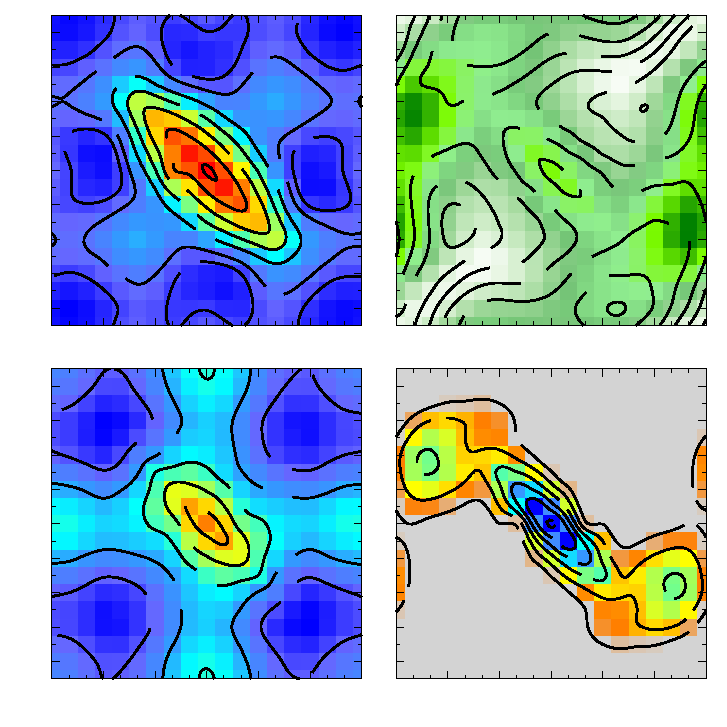
\includegraphics[width={349.00bp},height={349.00bp}]{Q0_maps}}%
    \gplfronttext
  \end{picture}%
\endgroup
